\section{Do isolated effects predict the full intervention?}
\label{sec:nonadditive}
We used the calibrated preferences on 2,400 summer markets: 100 fresh blocks, four boroughs, three months and two sampling protocols. For each higher-income renter $h$ we ran DA without $h$, then inserted $h$ at each feasible singleton, retaining the resulting displacement labels. When measuring this isolated change every other renter kept their baseline uniform recommendations. We computed $\delta_h$ for the realized uniform list and the transparent score's list. The conditional expectation over $h$'s uniform draw uses the binomial probabilities above. Each intervention has a separately verified endpoint. We express the sum of isolated count changes and the actual joint change on the same standardized lower-income match-rate scale. This diagnostic was designed after observing the joint effects on these draws.

\begin{table}[t]
\caption{One group changes its recommendations. The first numeric column sums its members' isolated effects against the same realized baseline. The last is the paired difference between joint and isolated effects, in percentage points. Every lower-income renter keeps the same list.}
\label{tab:isolated}
\centering
\begin{tabular}{@{}llrrr@{}}\toprule
Market draw & Score price penalty & Isolated sum & Joint change & Difference (95\% interval)\\\midrule
Ordinary & 1 & $+0.29$ & $+1.09$ & $+0.80$ $[0.53,1.06]$\\
Ordinary & 4 & $-1.44$ & $-0.31$ & $+1.14$ $[0.75,1.53]$\\
Enriched & 1 & $+7.25$ & $+13.72$ & $+6.47$ $[5.42,7.54]$\\
Enriched & 4 & $-1.44$ & $+9.03$ & $+10.47$ $[9.40,11.54]$\\\bottomrule
\end{tabular}
\end{table}

In enriched markets at score weight 4, adding the exact isolated changes predicts a 1.44-point loss ($[-2.65,-0.21]$). Switching all editors together produces a 9.03-point gain ($[8.58,9.49]$). Integrating exactly over each focal applicant's own uniform draw while holding peers fixed also gives a negative sum ($-2.10$ points). Some of the same incumbents can contribute a loss to several isolated experiments, and a later change can release an option that an earlier change left unavailable. The positive interaction residual measures the aggregate departure from additivity. It does not assign that residual to a unique chain.

To see how the two endpoints can coexist, we estimated $\Phi(p)-\Phi(0)$ from 24 random editor orders per market. At each prefix we know the effect of switching exactly that set. Given independent adoption probability $p$, the number switched is binomial, and conditional on that number every subset is equally likely. We combine the observed prefix outcomes using those exact binomial weights. The endpoint and the initial derivative also admit the exact calculations above. Figure~\ref{fig:rollout} keeps the other high-income renters' behavior endogenous to DA as the fraction of switched lists increases. Around 5--10\% adoption the enriched effect at weight 4 is close to zero and its pointwise interval includes zero. At 50\% adoption the gain is 2.47 points ($[2.18,2.75]$). We do not estimate an exact crossing point.

\begin{figure}[t]\centering
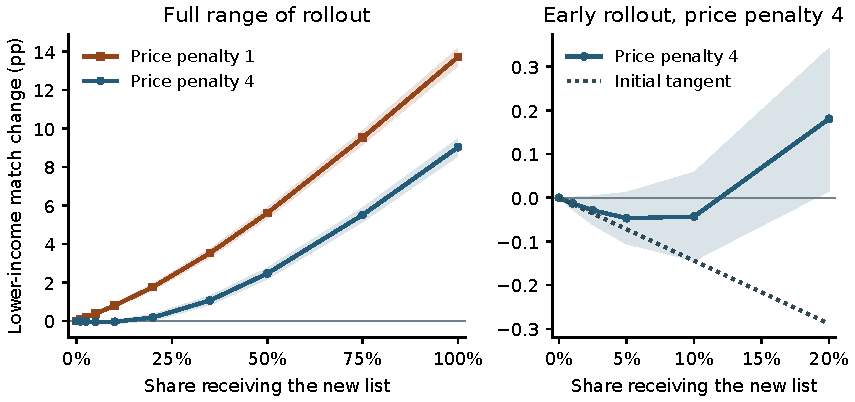
\includegraphics[width=.91\linewidth]{figures/rollout.pdf}
\caption{Partial rollout of the higher-income scoring rule in enriched five-listing markets. Shading gives pointwise 95\% block-bootstrap intervals. The dotted tangent is the exactly computed sum of the isolated effects at weight 4. The right panel enlarges early adoption.}
\label{fig:rollout}\Description{At score weight 4 the estimated gain is near zero early and rises to nine points by full adoption. The initial tangent is negative. At score weight 1 the effect is positive.}
\end{figure}

The experiment used 3,402,151 singleton insertions. On the first complete seed block 34,265 direct reruns checked singleton and score outcomes. Every realized baseline focal assignment agreed with the menu. The identities of matched lower-income renters agreed with residual-market DA for every score endpoint in every market. Switching editors in either forward or reverse order reproduced the final assignment and its total match change by summing successive, context-dependent changes. Separate exhaustive tests on 136,727 strict profiles across all labeled $2\times2$, $2\times3$, $3\times2$ and $3\times3$ feasible graphs checked the coalition identities and individual predictions. The archive also includes every market-level count used here.

\subsection{Does the scoring effect carry to another season?}
In the summer ordinary markets, holding rankings fixed at $(4,0.50)$ and varying only higher-income scoring weights $1,2,4$ gives lower-income spillovers of $+1.09,+0.49,-0.31$ points. A separate family of 36 simultaneous intervals excludes zero for each of those three comparisons. At a five-listing quota competitor-score changes can therefore reverse the effect on the fixed group even without changing rents or applicant tastes.

For a temporal check we fixed the January--March 2026 score comparison and its primary outcome before running this specific intervention. These months had been examined earlier under a simpler cheapest-first rule. They are fresh dates relative to summer calibration but not previously unseen catalogues. We froze summer quality, geography and price references and used the same calibration household pool. Using the calibrated cleaning rules across four boroughs gave 47,873 eligible winter records. We excluded 2,100 identifiable summer overlaps, 1,059 winter repeats and 24 ambiguous identities. All twelve winter cells supported both sampling designs. Eighty new blocks produced 1,920 markets and 11,520 DA outcomes. We also checked 288 entire assignment vectors against a second algorithm.

\begin{table}[t]\centering
\caption{Winter lower-income match rates, with each lower-income list fixed. The last column is the difference between the two scoring rules, with a simultaneous interval across twelve winter contrasts.}
\label{tab:winter}
\begin{tabular}{@{}llrrrr@{}}\toprule
Market draw & Quota & All uniform & Higher $T_1$ & Higher $T_4$ & $T_1-T_4$ (points)\\\midrule
Ordinary & Five & 3.07\% & 4.57\% & 2.56\% & $+2.01$ $[1.77,2.25]$\\
Ordinary & 40\% & 2.02\% & 3.19\% & 1.60\% & $+1.58$ $[1.32,1.84]$\\
Enriched & Five & 39.90\% & 53.08\% & 48.76\% & $+4.32$ $[3.92,4.72]$\\
Enriched & 40\% & 38.22\% & 43.70\% & 36.75\% & $+6.95$ $[6.52,7.38]$\\\bottomrule
\end{tabular}
\end{table}
The ordinary top-five spillover relative to uniform was $+1.50$ points at scoring weight 1 and $-0.51$ at weight 4. The preselected comparison \emph{between} scoring rules was $+2.01$ ($[1.85,2.18]$ pointwise). The result recurs in a different season with summer behavioral assumptions held fixed. The two seasons cannot establish how renters actually trade off price against other attributes.
